\documentclass[a4paper]{report}
\usepackage[utf8]{inputenc}
\usepackage{tikz-uml}
\usepackage{tikz}
\usepackage{notoccite}
\usepackage{hyperref}
\usepackage{graphicx}
\usetikzlibrary{fit,arrows,calc,positioning}
\usepackage{titlesec}
\usepackage{amsmath}
%\usepackage[margin=1in]{geometry}
%\usepackage[tmargin=1in,bmargin=1in,lmargin=1.25in,rmargin=1.25in]{geometry}
%\usepackage{natbib}
\usepackage[round, sort, numbers]{natbib}\usepackage{graphicx}
\usepackage{url}
\usepackage{lipsum}
\usepackage{etoolbox}

\newcommand{
	\subsubsubsection}[1]
{\paragraph{#1}\mbox{}\\[.35em]}
\setcounter{secnumdepth}{4}
\setcounter{tocdepth}{4}

\titleformat{\chapter}[display]   
{\normalfont\huge\bfseries}{\chaptertitlename\ \thechapter}{20pt}{\Huge}   
\titlespacing*{\chapter}{0pt}{-50pt}{40pt}

\begin{document}
	\begin{titlepage}
		\newcommand{\HRule}{\rule{\linewidth}{0.5mm}} % Defines a new command for horizontal lines, change thickness here
		\newcommand{\hRule}{\rule{\linewidth}{0.1mm}} % Defines a new command for horizontal lines, change thickness here
		\centering
		
\includegraphics[width=0.2\textwidth]{kcl.png}\par\vspace{1cm}
		\textsc{\LARGE King's College London}\\[1.5cm] % Main heading such as the name of your university/college
		\textsc{\large 7CCSMGPR}\\[0.5cm] % Major heading such as course name
		\textsc{\Large Group Project}\\[0.5cm] % Minor heading such as course title
		\HRule\\[0.4cm]
		{\huge\bfseries Team of Seven Report}\\[0.4cm] % Title of your document
		\HRule\\[1.5cm]
		\vspace{1cm}
		\textit{Authors: }\vspace{0.5cm}
		\begin{center}
			\begin{tabular}{ c|c|c } 
				\hline
				\textbf{Number} & \textbf{Name} & \textbf{Email} \\
				\hline
				1756850 & Othman \textsc{Alkhamra} &  othman.alkhamra@kcl.ac.uk \\ 
				\hline
				1739256 & David \textsc{Benicek} &  david.benicek@kcl.ac.uk \\ 
				\hline
				1770922 & Aadam \textsc{Bari} &  
				aadam.bari@kcl.ac.uk\\ 
				\hline
				1425704 & Hitesh \textsc{Mankani Vinod} &  hitesh.mankani\_vinod@kcl.ac.uk \\ 
				\hline
				1755013 & Timothy \textsc{Obimma} &  timothy.obimma@kcl.ac.uk \\ 
				\hline
				1783087 & Nagarjuna \textsc{Vaddiraju} &  nagarjuna.vaddiraju@kcl.ac.uk \\ 
				
				\hline
			\end{tabular}
		\end{center}
		
		\vfill
		supervised by\par
		Dr.~Laurence \textsc{Tratt}\par
		Word count: 11236
		\vfill
		{\large \today\par}
	\end{titlepage}
	% \maketitle
	\newpage
	\pagenumbering{roman}
	\tableofcontents
	\newpage
	\pagenumbering{arabic}
	\chapter{Introduction}
	%In this section: Describe the context for the work and the problem you are addressing. Briefly summarise what you achieved in the project.
	Over the last several years, photo realistic digital imagery has become a mainstream technology. Computer graphics are now at a stage where they closely resemble real-world objects and trends such as mixed, augmented and virtual reality are supercharging that paradigm shift. Ray tracing is one of the many techniques that are used to produce different images, video renderings, games and animations. In this project, we implemented our own version of a ray tracer that is able to render multiple simple objects inside a user-defined scene. 
	
	\section{What is the Idea behind  Ray Tracing?}
	
	Before discussing the algorithms behind ray tracing and diving into details of our project let us begin with listing the basic required elements to run the ray tracing algorithm. In real life, we have different objects such as spheres, cubes, polygons etc. What's mutual between them is that they are all geometry objects. Those objects might appear in different ways, based on their environment and their combinations. A mirror sphere placed in an environment with many light sources will for example react and appear vastly different than a metal sphere would. Due to the multiple factors that influence  the appearance of a scene and the objects within it, we must take the following elements into account:   
	\begin{itemize}
		\item \textbf{Object(s)}: a scene can contain one or many objects. In real life, objects can be absolutely anything (cars, houses, trees...), however, for the purposes of this project, we are only going to consider simple geometric objects such as spheres, cubes or planes.
		\item \textbf{Light source(s)}: The algorithm of ray tracing itself doesn't require having a light source, however, a scene without any light source isn't very practical for ray tracing. Furthermore, each light source is likely to influence how a scene is rendered in substantial ways and therefore it's a necessary element to consider.
		\item \textbf{Image Plane}: referred to as window frame in our implementation. This plane has a set width and height and is divided into small squares, where each square covers a number of pixels on the objects of the scene.
		\item \textbf{Eye or Camera:} In order to render the scene, it is mandatory to have an eye or camera, with a certain position and direction. The camera is used to determine the way of looking at the scene elements. From the eye or camera, view rays are produced which travel through the image plane and determine the way the object is rendered.
		
	\end{itemize}
	\begin{figure}[ht!]
		\centering
		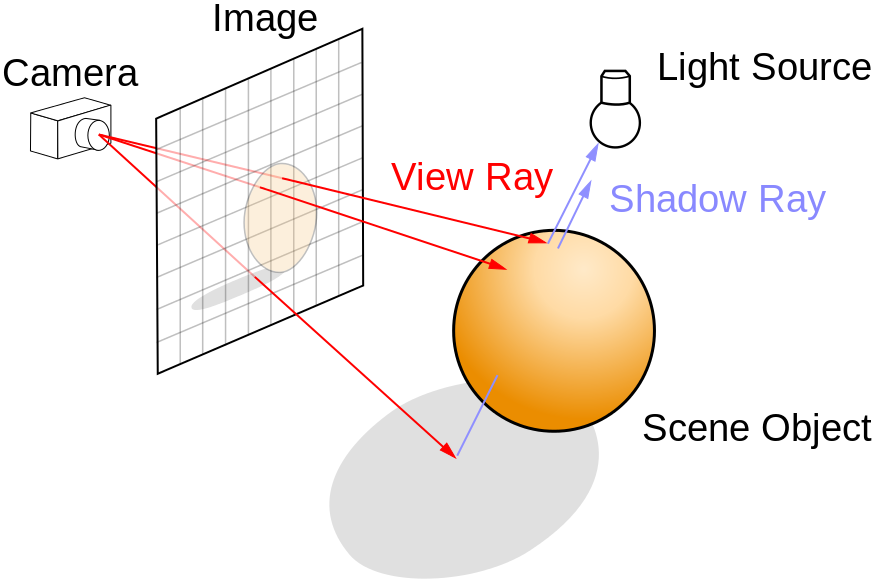
\includegraphics[scale=0.2]{./raytracing.png}
		\caption{Ray Tracing's Scene Elements \cite{scratchapixel_overview_2014}}
		\label{fig:raytracing}
	\end{figure}
	\par \textbf{Figure \ref{fig:raytracing}} shows an example of a scene with the previously listed elements. Despite the implementation not being trivial, the main idea is quite simple; in each scene, there will be an eye or camera from which many rays will be produced and go across the small squares in the image plane. For each ray, we check whether it intersects with any of the objects in the scene or not, and return the colour of that pixel. Rays, other than the initial camera rays, are produced by reflection. These rays also follow the ray tracing algorithm before returning the final colour. Even though the algorithm itself is relatively simple to describe, environment variables play a big role in the calculations and as a result, returning the colour of a pixel, which was hit by a certain ray, is not nearly as simple since it requires additional computations related to the reflections, shades etc.
	
	\section{Our Solution}
	Over the course of the project, we worked hard to deliver a final product that is able to render a scene created by the end-user using a web interface. The web interface provides both 2D and 3D views, where the user can create his own scene, and then just click render. After that, the user's input will be processed by the back end engine, which in turn returns the rendered image as a PNG file, with the name chosen by the end-user, back to the front end.\newline  
	
	\par The scene can contain multiple objects of two different supported object types, each constituting of any of the six available materials in our program. In addition to that, the scene can have multiple light sources. Further information on how each of these is implemented and present to the user can be found in \textbf{Chapter \ref{ch:imp}}.\newline
	
	\par Our solution showed great results for the inputs we defined, and in order to make our product more reliable, we covered both the front and the back ends with many tests. More details about the implementation and testing will be discussed later in \textbf{Chapter \ref{ch:imp}}.
	
	\chapter{Review}
	\section{Brief History of Ray tracing}
	
	\par Digital photo-realistic images are usually generated by rendering a 2D or 3D model based on a set of inputs and ray tracing is one of the prominent approaches that is used to achieve this. There are, in total, three similar techniques to image rendering and they are rasterisation, ray casting and ray tracing. These three techniques are differentiated by their representation of the optical effects such as reflection and intensity, which impacts the end result and the processing speed \cite{wald_interactive_2001}. Ray tracing produces the most photorealistic image while also taking the most time to compute while rasterisation produces a more basic image but is generally faster.\newline
	
	\par The earliest known Ray tracing system was calculated by hand by Richard Hoyt in the 1950s while working on vehicle shotline at the Ballistic Research Library, known today as DARPA \cite{klopcic_historical_1999}. In the 1960s, physicists coined the name "ray tracing" by plotting on paper the path taken by rays of light starting at a light source and passing through the lens in the design of lenses \cite{glassner_introduction_1989}.\newline
	
	\par Computer Graphics researchers at the University of Utah thought it would be a good idea to apply this simulation of light physics to create images, however, the computers of the 1960's were too slow to produce images of better quality than those made by using cheaper image rendering techniques. As a result of the processing intensity of ray tracing, the idea was dropped for several years, only to be revisited later as computer grew more powerful and became capable of simulating real physics\cite{weghorst_improved_1984}. Since then, several optimised algorithms were implemented and this led to computers being able to simulate various kinds of optical effects. Ray tracing has evolved greatly over the following years and it is now one of the most powerful techniques used in image rendering. Ray tracers have become both faster and more efficient and can even produce hyper-realistic images that are indistinguishable from the real world. We will Discuss some notable Ray tracers in Section \ref{sec:review-of-tracers}.\newline
	
	
	\section{Overview of Ray Tracing}
	\par Ray tracing is a simple yet powerful technique. It involves shooting rays from a point-of-view (usually represented by an eye or a camera) which then go through each pixel of the viewing plane while calculations are done to determine if they intersect with objects. When an intersection is detected, reflected or refracted rays are generated \cite{weghorst_improved_1984}. Each of the reflected/refracted rays must be recursively calculated to determine which surfaces they intersect. At each pixel where the intersection occurs, the ray tracer must work out the intensity of the light and how much of it is reflected back in order to determine the exact colour of the pixel \cite{suffern_ray_2007}. This is usually a long process and the time taken to generate each image increases exponentially with respect to an increase in the size of the viewing plane(image frame).\newline
	
	\section{Review of Related Work} \label{sec:review-of-tracers}
	\par The ray tracer discussed in this section helped inform our design decisions and served as an inspiration for the structure of our own ray tracer.
	
	\subsection{Ray Tracing from the Ground Up}
	\par The ray tracer described in this book was developed using Object-Oriented(OO) techniques due to its size and complexity. Ray tracers are incredibly large and complex and as a result, the tools provided by OO techniques such as inheritance and polymorphism are extremely useful as they enable extensibility and allow us to use existing code to handle different types of object. The book uses C++ as its development language because of its OO facilities and its computational efficiency. Some useful coding tips such as data storage, references and floating-point division were also gathered from this book though we would go on to implement our solution in C\#. Important mathematical calculations such as sets, vectors, points, normal and the operations that can be carried out among them are also discussed extensively in this book \cite{suffern_ray_2007}.
	%     \texorpdfstring{\cite{suffern_ray_2007}}{}
	%     \nocite{suffern_ray_2007}
	\label{sssec:book}\newline
	
	\par The book focuses on the Ray Tracing engine (i.e. the back end) and largely ignores any form of user-interface. The necessary inputs such as objects, material, light and frame size are hard-coded. The workings of the ray tracer described in the book can be represented using the pseudo-code below:\newline
	\begin{itemize}
		\item Add the objects to be rendered
		\item Add the type of material each object possesses
		\item Add the source(s) of light 
		\item Add a plane which is made up of pixels
		\item Per individual pixel:\newline
		Trace a ray in the direction of the object from the pixels centre.\newline
		Compute the closest point of intersection of the ray with an object (if any exists)
		\begin{itemize}
			\item If an object is hit by a ray
			\par Calculate the colour of a pixel using the material of the object as well as the light 
			\item Else
			\par The default colour of the pixel is the background colour\cite{suffern_ray_2007}. 
		\end{itemize}
	\end{itemize} 
	
	\par Colours are represented using their RGB value which is then stored in a 3D colour space. This allows various calculations to be carried out in order to produce an extensive variety of colours. See \textbf{Figure \ref{fig:colour}} for representation of pure Red, Green and Blue.
	
	\begin{figure}[ht!]
		\centering
		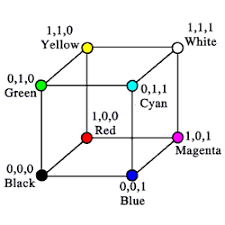
\includegraphics[scale=0.60]{./colour.png}
		\caption{RGB colour scheme}
		\label{fig:colour}
	\end{figure}
	
	\par The book also discusses the bounding-box technique. This technique is used to improve efficiency when an object is expensive(this refers to non-conventional shapes or objects such as animals or figures) to trace. This method only saves time if the bounding box is significantly cheaper to intersect than the object inside such as in \textbf{Figure \ref{fig:boundingbox}} below. It works by enclosing the object in a rectangular box and when running the ray tracer, it first checks if a ray misses the bounding box, then it cannot hit the object inside \cite{suffern_ray_2007}. We did not implement this technique as our ray tracer only supports simple objects at this time however it could be a future improvement.
	
	\begin{figure}[ht!]
		\centering
		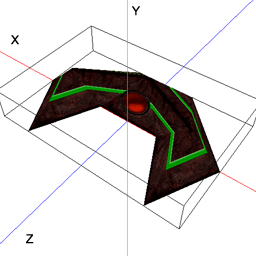
\includegraphics[scale=0.60]{./boundingbox.png}
		\caption{Bounding Box Example}
		\label{fig:boundingbox}
	\end{figure}
	
	\chapter{Requirements and Design} 
	%In this section: Describe the requirements you set for your project at the beginning and the design you have taken for your project. Focus on why you decided to tackle the problem in the way you did, and what effects that had on the design. You may also wish to mention the impact of team-working on your requirements and design.
	\label{chapter:requirements}The very first stage of software engineering is requirements elicitation. The initial set of requirements for our project were informed partly by the literature that we have reviewed and also by the description of the project given to us by Dr. Tratt. These simple requirements were not enough, and so we analysed the possible requirements that we could add in order to enhance both user experience and the usefulness of the project in general. From this analysis, we ended up with a set of mandatory and optional requirements.\newline
	\par As we are following an agile methodology, we performed the design stage, then moved to the implementation, wrote some tests for each sprint of requirements and goals. All the software engineering stages and steps will be explained and described in more details in the Chapter \ref{chapter:teamwork}.
	
	\section{Mandatory Requirements}
	
	At the beginning of the project, the group discussed and decide what features were essential for the ray tracer to function. This debate covered what is needed to create and develop a functioning system, consisting of a client side and a back end server. The minimum requirements for the entire system were determined to be as follows:
	\begin{itemize}
		\item Allow users to create spheres and cubes with specific parameters values. Those parameters are:
		\begin{itemize}
			\item The size of the object.
			\item The position of the object.
			\item The material of the object; determining its colour and translucency.
		\end{itemize}
		\item Allow users to assign values to the parameters of the environment. The parameters include the following:
		\begin{itemize}
			\item Position of the camera.
			\item Size of the output image and the window frame.
			\item Filename of the output image.
			\item Colour of the background.
			\item Light's colour and position.
		\end{itemize}
		\item Render multiple objects in the same scene, with at most one light source.
	\end{itemize}
	
	\section{Optional Requirements}
	
	The group established additional requirements that were deemed a lower priority and would be completed if time allows.
	The requirements specified in this category will extend the basic functionality of the ray tracer, thus distinguishing our product from others. The optional requirements are as follows:
	\begin{itemize}
		\item Allow users to add multiple lights to the scene in different positions, colours and intensities.
		\item Provide users with a drag and drop user interface to build the scene
		\item Provide users with a 3D approximation of the final scene on the front end
		\item Allow users to create other objects such as polygons.
		\item Allow users to choose different materials, such as plastic, mirror, etc. for the objects.
		\item Improve the colours of the output image, by using different techniques such as sampling.
		\item Improve the performance of our system, by applying the multi-threading concept, if the system takes a long time while rendering the scene.
	\end{itemize}
	
	\section{Architecture}
	\label{sssec:arch}
	The project task involved developing the ray tracing engine and the GUI as distinct components which interacted with each other over a well defined interface.
	
	A decision was made to use the ASP.NET technology, which made it extremely easy for the group to take advantage of the ASP.NET MVC web application framework. The different components of this framework are designed in such a way that they can be easily replaced or customised independently without effect on other components \cite{microsoft_asp.net_2018}. The .NET framework implements the Model–View–Controller pattern and allowed us to divide the application into a composition of three main logical components: Model, View and Controller which represents the Business logic, UI logic and Input logic respectively. Each of the components is loosely coupled with the other but tightly aligned to make sure they work together nicely. By using such an architecture we were able to develop multiple sections of the system at once and thus easily divide up the labour. 
	
	\tikzstyle{b} = [rectangle, draw, fill=gray!20, node distance=3cm, text width=7em, text centered, minimum height=4em, thick]
	
	\begin{figure}[ht!]
		\centering
		%         \includegraphics[scale=0.15]{./mvc.png}
		\begin{tikzpicture}[->,node distance=2.5cm,auto,main node/.style={rectangle,rounded corners,draw,align=center}]
		\node [b] (model) {Model};
		\node[b] at (-3, -3) (view) {View};
		\node[b] at (3, -3) (controller) {Controller};
		\node[b] at (3, -3) (controller) {Controller};
		\node[b] at (0, -7) (user) {User};
		\path[scale=1.3, ->, thick, solid] 
		(model) edge[bend right=45 line width=1mm] node[ fill=white, anchor=center, pos=0.7,font=\bfseries] {UPDATES} (view)
		(controller) edge[bend right=45] node[ fill=white, anchor=center, pos=0.3,font=\bfseries] {MANIPULATES} (model)
		(view) edge node [ fill=white, anchor=center, pos=0.5,font=\bfseries] {SEES} (user)
		(user) edge node[ fill=white, anchor=center, pos=0.5,font=\bfseries] {USES} (controller);
		\end{tikzpicture}
		\caption{Model View Controller Architecture}
		\label{fig:mvc}
	\end{figure}
	
	\begin{itemize}
		\item \textbf{Model} - The Model component corresponds to the back end and contains all of the business logic. This component is responsible for manipulating all data transferred between the View and Controller components as well as the rules and logic associated with the system. In our system, this is the ray tracing engine that performs all of the calculations and determines if a ray hits an object as well as its colour, shadow, etc \cite{tutorialspoint_mvc_2018}.The data used in this component is gotten from the controller.\newline
		
		\item \textbf{View} - The View component is used for all the UI logic of the application. This represents the interface that the user interacts with. In our case, this is represented by the front end which includes an interactive SVG (where users can drag and drop objects as well as move them around), a 3D view which gives actual representation of the scene (including depth) and a form which is used to include additional details such as scene size, light position/intensity, point-of-view, etc. \cite{tutorialspoint_mvc_2018}\newline
		
		\item \textbf{Controller} - The Controller acts as an interface between Model and View components. It receives input from the View, converts it to understandable commands for the Model. In our system, the controller is represented by an API that extracts data objects from a JSON file and transmits them to the back end. The controller is extremely useful as it also validates the input from the user. \cite{tutorialspoint_mvc_2018}
	\end{itemize}
	
	
	\section{Prototypes} \label{sec:prototypes}
	We produced prototypes to visualise the design of our web page and to evaluate its strengths. Its also assisted us in identify specifications for our system. 
	
	\subsection{First Iteration}
	
	Our first iteration was a low fidelity prototype drawn by hand to represent what the homepage might look like. This prototype reflects our early assumptions about the system and the inputs required for the ray tracer back end to operate. The simplicity of this prototype (in that it is a simple form) also reflects our early intention of usability, that is to say, keeping the system usable for the user. We had initially desired to keep development process simple also and a form seemed the simplest way to deliver the front end component of the project fulfilling the basic requirements.
	
	\begin{figure}[ht!]
		\centering
		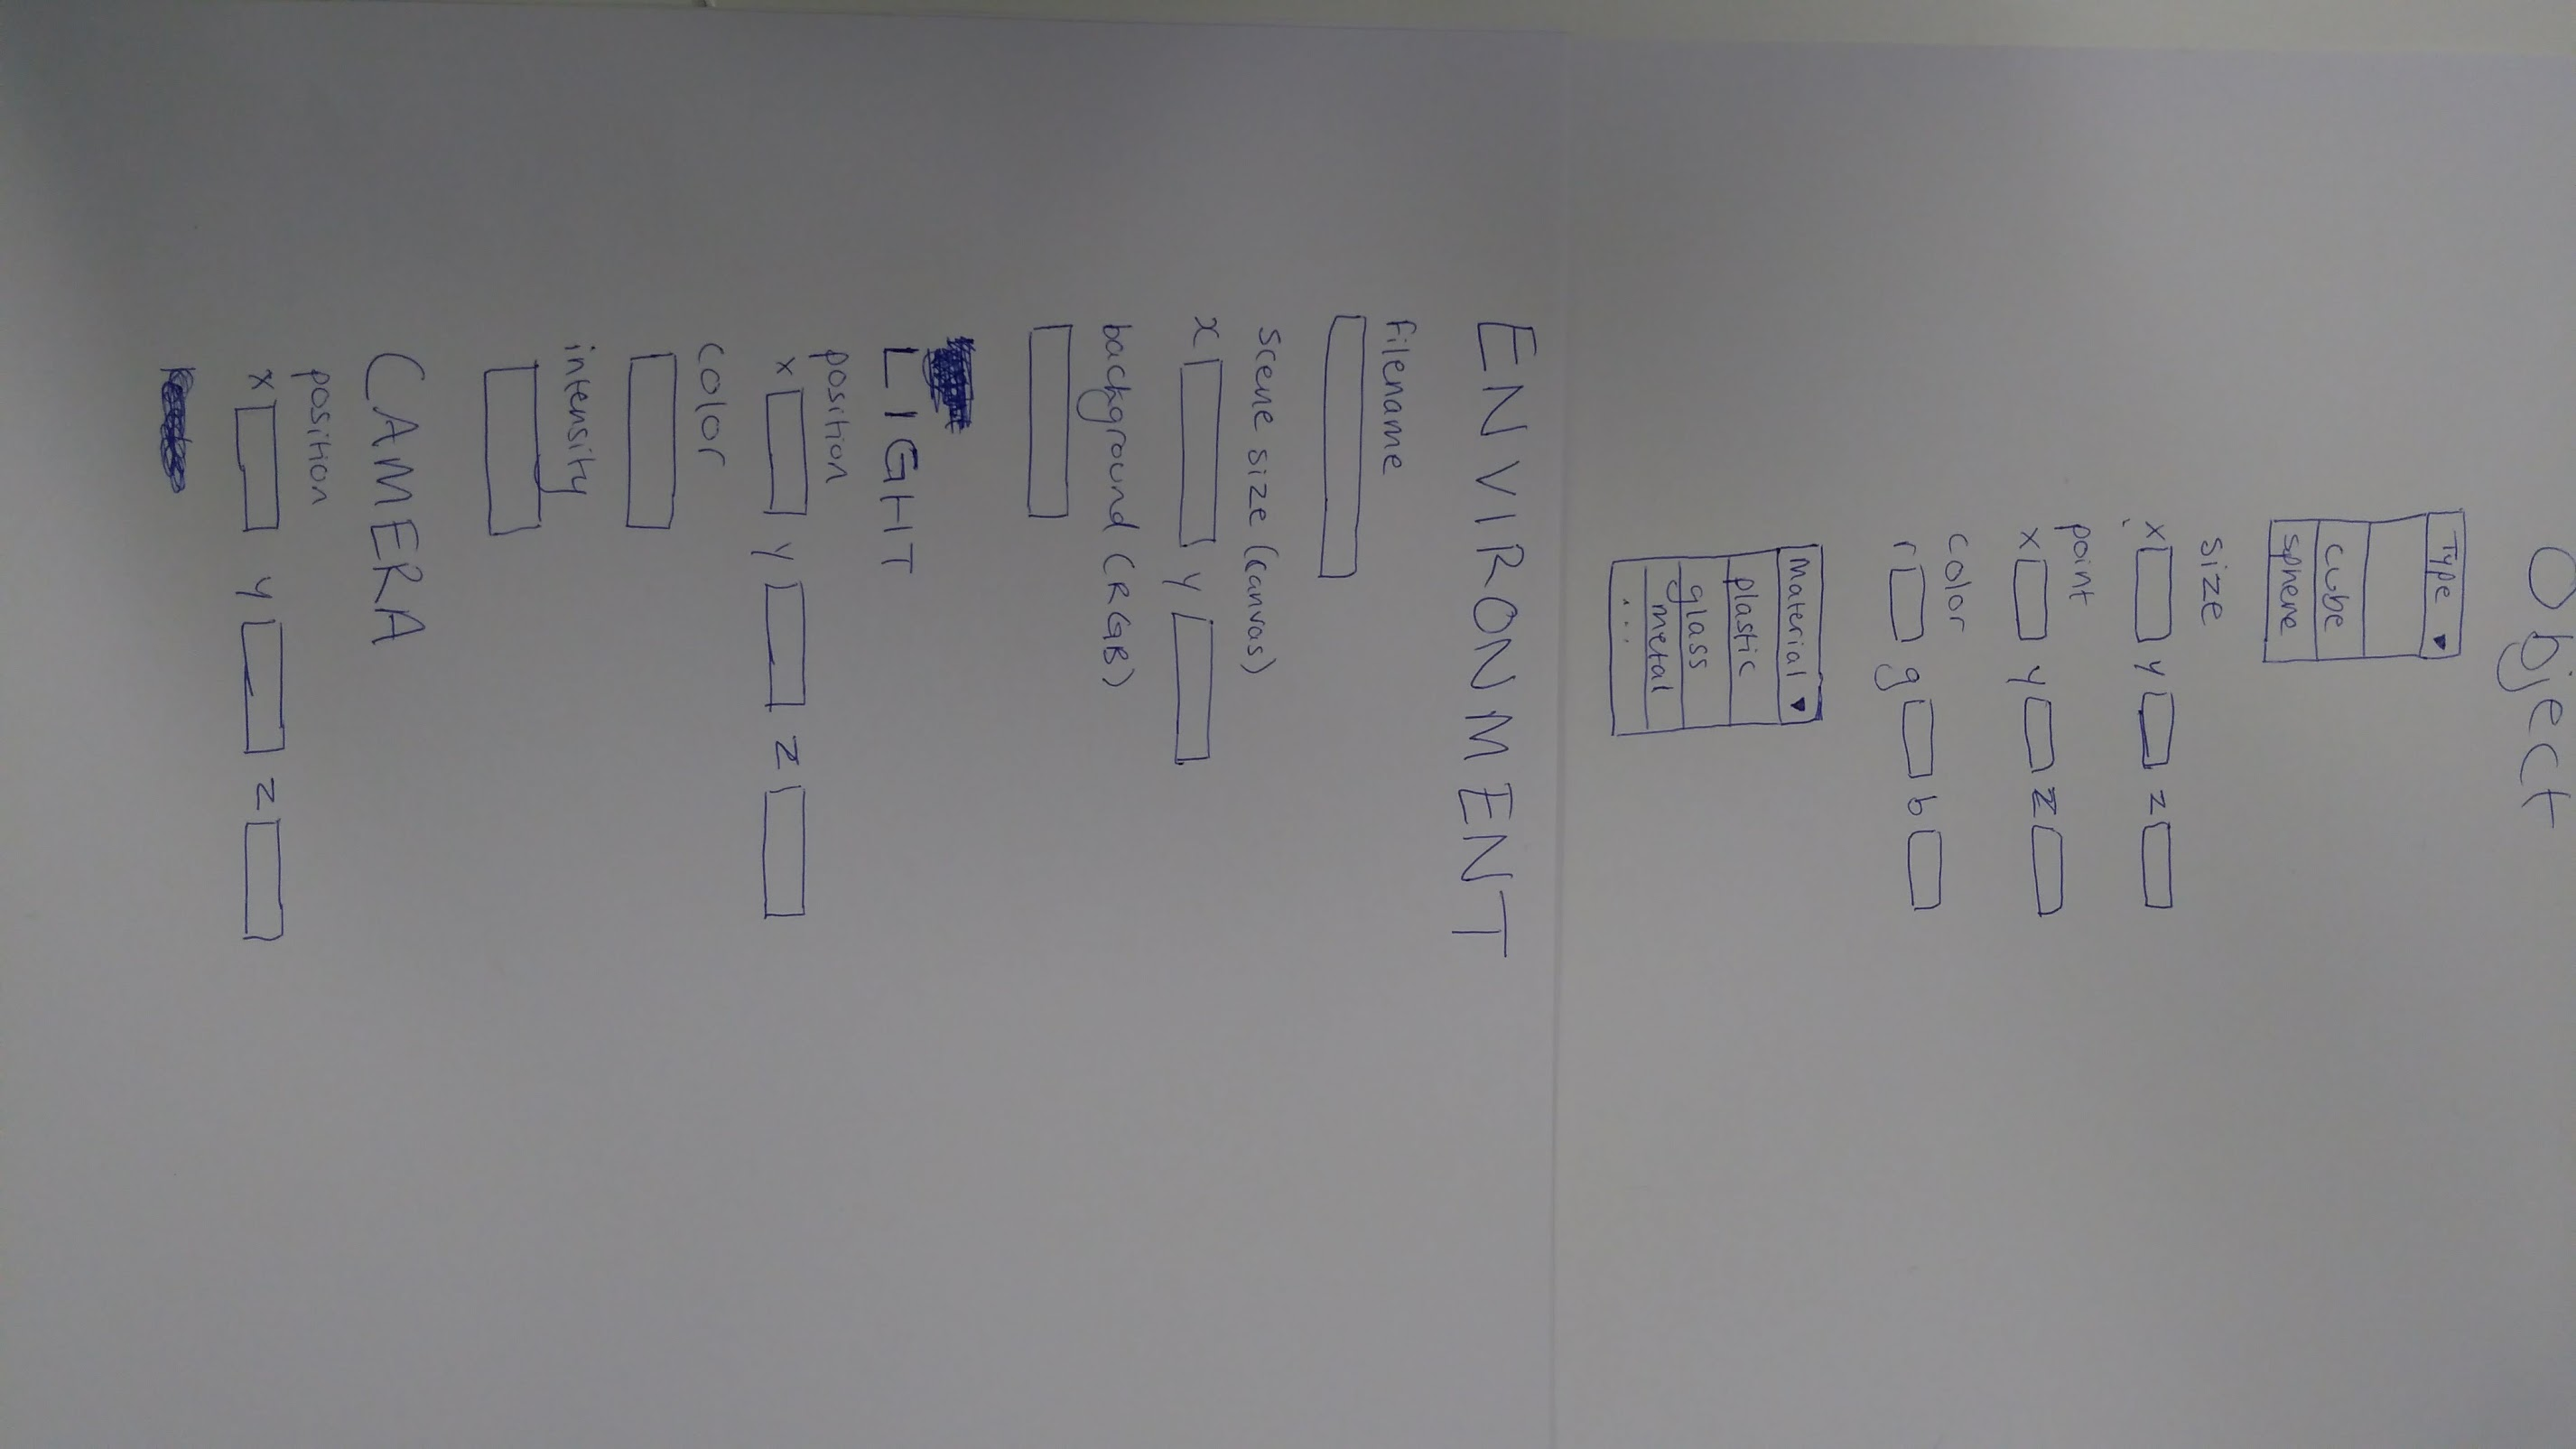
\includegraphics[angle=90, scale=0.1]{First_Iteration_Prototype.jpg}
		\caption{First Iteration}
		\label{fig:firstIt}
	\end{figure}
	
	\subsection{Second Iteration}
	
	Our second iteration was a medium fidelity prototype which included our evolved requirements for the project. This prototype demonstrates the change in our outlook of how we should present the front end of the system. As mentioned above, we were initially concerned with usability and ease of development, however, at this stage, we decided to focus on ease of use in favour of ease of development. We aimed to be more ambitious than producing a merely \textit{use-able} system, rather we endeavoured to deliver an advanced and high functioning graphical user interface that ensured accessibility for the users. This design visualises a shortened version of the form and how our GUI, (in the form of a drag and drop SVG interface), would appear and we believed this would be far more practical than a time-consuming form.
	
	\begin{figure}[ht!]
		\centering
		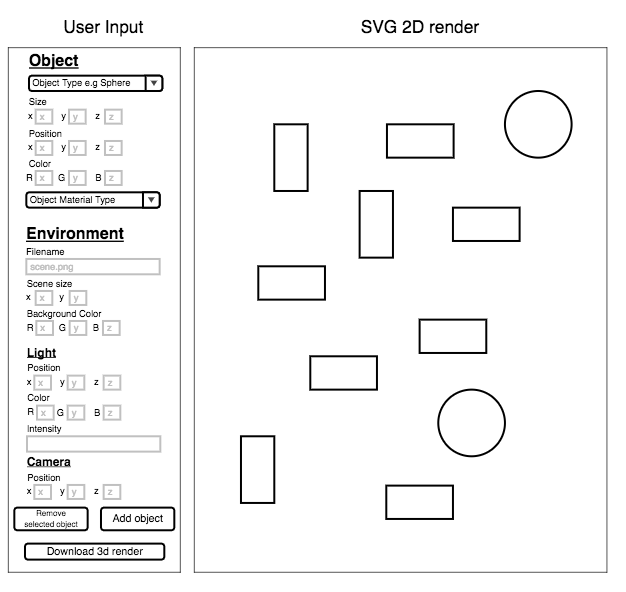
\includegraphics[scale=0.8]{second_prototype.png}
		\caption{Second Iteration}
		\label{fig:secondIt}
	\end{figure}
	
	\subsection{Final Iteration}
	
	Our final iteration and high fidelity prototype reveals our end product. The only substantial difference in design is the fact that the object specification appears in a popup box as opposed to appearing in the form. We believe this is more intuitive for the user in that the pop up appears next to the (SVG) shape clicked on, allowing them to modify individual shapes and customise exactly what the intended output of the ray tracer is. The contrast in the length of the form is very apparent here between the final and first iteration of our prototypes.
	\begin{figure}[ht!]
		\centering
		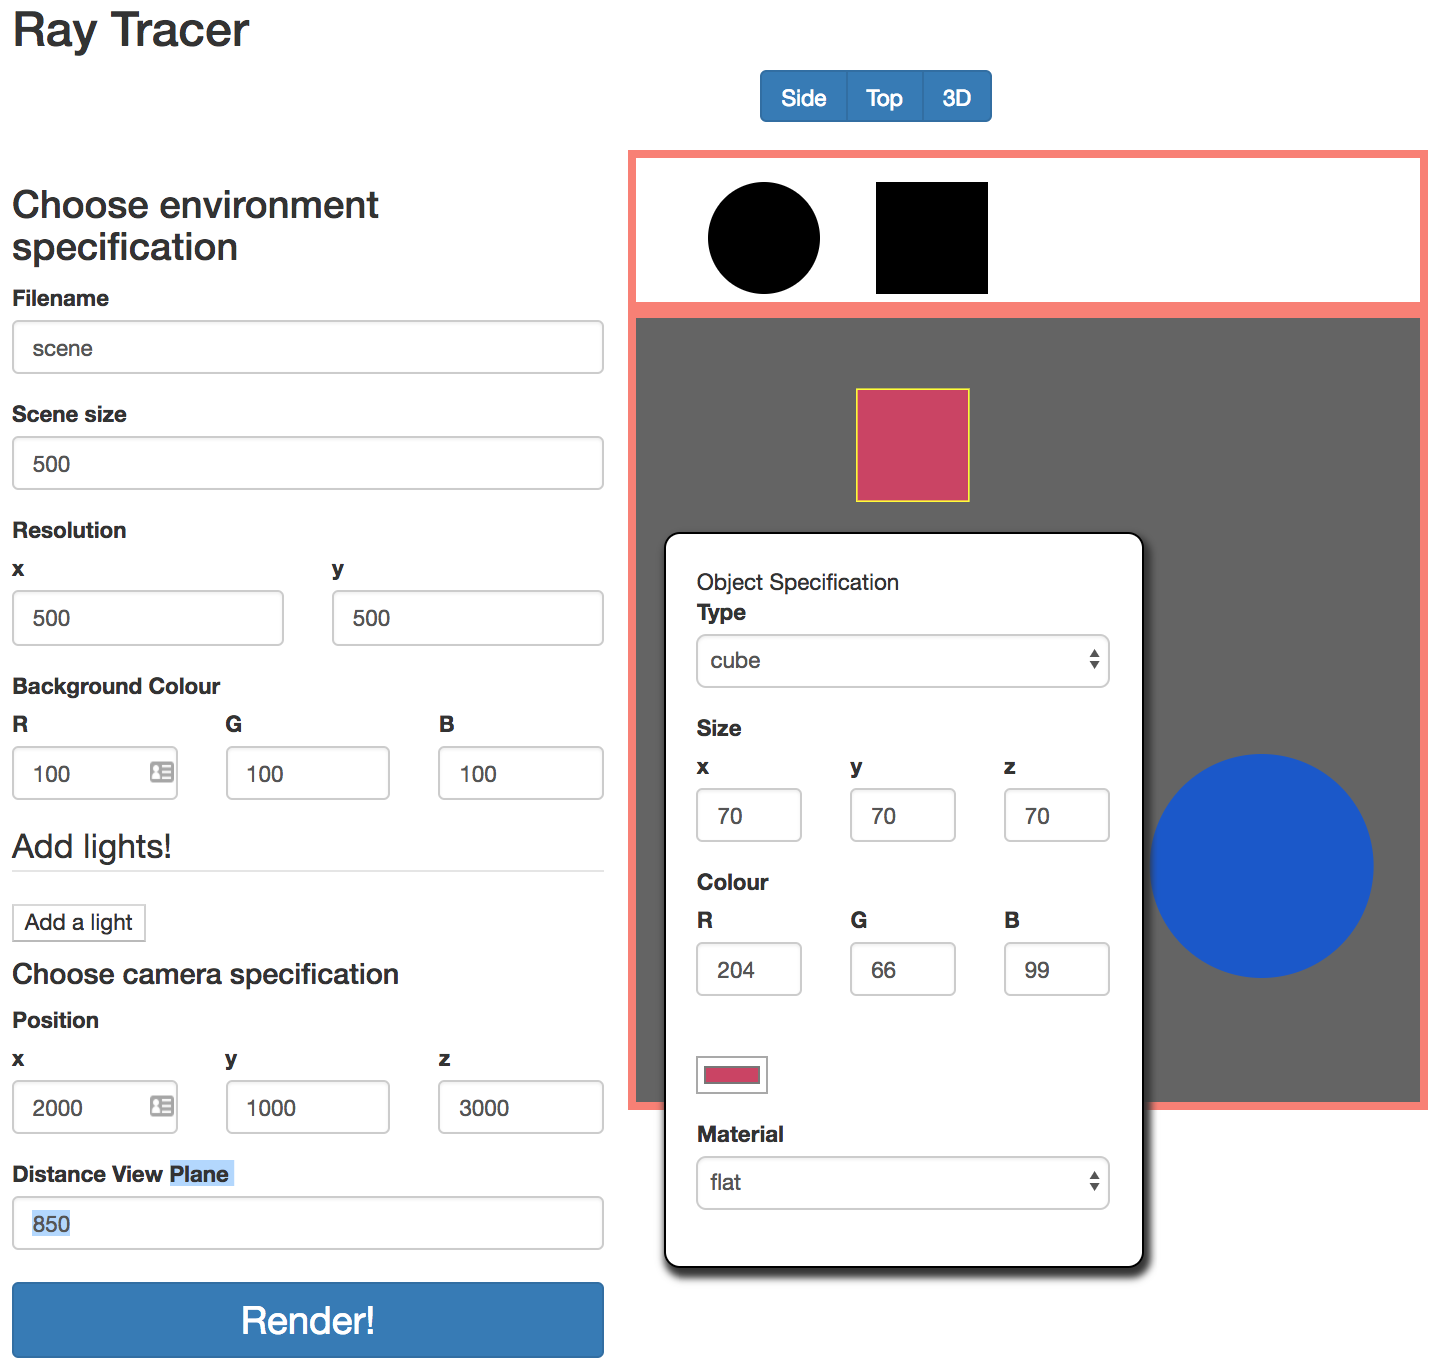
\includegraphics[scale=0.3]{final-all.png}
		\caption{Final Iteration}
		\label{fig:final}
	\end{figure}
	\chapter{Implementation}
	
	%In this section: Describe the most significant implementation details, focusing on those where unusual or detailed solutions were required. Quote code fragments where necessary, but remember that the examiners have full access to your source code. Explain how you tested your software (e.g. unit testing) and the extent to which you tested it. If relevant to your project, explain performance issues and how you tackled them.
	\label{ch:imp}\section{Back End}
	The code in the back end is inspired by the ray tracer solution covered in the book discussed in \textbf{Section \ref{sssec:book}}. As mentioned before, the ray tracing algorithm is mainly about checking if the ray hits/intersects with the object or not, which goes from the camera or reflects from objects because of lights. Furthermore, ray tracing depends on the material of each object; since not all materials will react in the same way to light sources - some materials absorb light, while others reflect it.    Therefore, we should take that into our consideration. In addition to that, each scene has lights and cameras, and since each of these can have a different type, we need to implement that to be scalable and open for extension.\newline
	\par In our implementation, we make use of different object-oriented principles such as abstract classes, inheritance, overriding and polymorphism. In the following sections, we will discuss in details how we used each of these concepts in our codes.
	\subsection{Models}
	Our architecture is mainly based on the MVC model as previously discussed in \textbf{Section \ref{sssec:arch}}. This section will introduce and discuss the models used in our system.
	\subsubsection{Basic Elements}
	There are many basic elements which are required to build a ray tracer. These elements were reflected in our project as classes: 
	\begin{itemize}
		\item \textbf{Point3D}: This class is used to create a point in the 3D with x,y and z double values. In this class, all the addition, subtraction, division and multiplication were overridden in order to perform them correctly in the context of points. Also, there are other methods such as the distance, which will be used to return the distance between two points.
		\item \textbf{Vector3D}: Vector3D is responsible for representing a vector in the 3D with x,y and z double values. In this class, all the addition, subtraction, division and multiplication were overridden in order to perform them correctly in the context of vectors. There are also other methods such as the length, which will be used to return the length of a vector. Furthermore, the dot and cross products methods were implemented; since they are crucial in our project.
		\item \textbf{ColourRGB}: ColourRGB is used to create a colour with R, G, and B double values. In this class, all the addition, subtraction, division and multiplication were overridden in order to perform them correctly in the context of colours.
		\item \textbf{Point2D}: This class is used to create a point in 2D with x and y double values. No other methods were added to this class; since they are not needed in this class.
		\item \textbf{Ray}: The Ray class is used to represent a ray, which will have an origin with a type of \textbf{Point3D}, and a direction with a type of \textbf{Vector3D}. This ray will be used in most of the calculations of ray tracing. There are no methods directly implemented in this class, but it will make use of other methods implemented in \textbf{Point3D} and \textbf{Vector3D}.
	\end{itemize}
	\subsubsection{Configurations}
	In order to make it easier to change any configured value in our program, we created a class called \textbf{Config}, where you can find any default values used in our program. By doing that, we make sure that changing the value in one place will change it in all the places where it is used. For example, the default colour, material, vector, point ... etc are defined in that class. 
	\subsubsection{Materials}
	\label{sssec:mat}One of the main factors which will affect the final result of ray tracing is the material of the object. All materials will have a colour, in addition to many different coefficients such as diffusion; specular; ambient, that might be needed for other materials. In each material, we need a method that will calculate the shades caused by lights and other objects. \newline
	\par It is clear that we need to have an abstract class with the previously mentioned attributes, in addition to an abstract method which will be called calculateShade, which will be implemented differently based on the material. In our solution, we covered three types of materials:
	\begin{itemize}
		\item \textbf{Phong materials}:  These materials follow what is called the Phong model. This model says that it is possible to create new materials and compute them as a sum of weighted specular and diffusion components. As a result, the reflection of lights by those materials is a combination of the specular and diffusion reflections. In our program, we have three different types of materials following that model which are: Chalk, Metal and Plastic. The difference between those materials is the values of diffusion, specular coefficients and the light colour influence \cite{scratchapixel_phong_2015}.
		\item \textbf{Flat material}: which is the simplest material, that will return the colour of that object regardless of any other environment variables and parameters.
		\item \textbf {Mirror material}: this material is the most complicated one because it is highly reflective and therefore produces many rays. As a result, many different calculations must be done in order to calculate the colour of each pixel of the object.
	\end{itemize}
	In our program, we implemented these three different types. However, for the phong material, we covered three different materials, which follows the phong model, and so we have six supported materials in total. Each of those materials can have a colour chosen by the user, or just use the default colour, if null. \textbf{Figure \ref{fig:matcd}} shows the class diagram of the supported materials in our program.
	a \begin{figure}[ht!]
		\centering
		%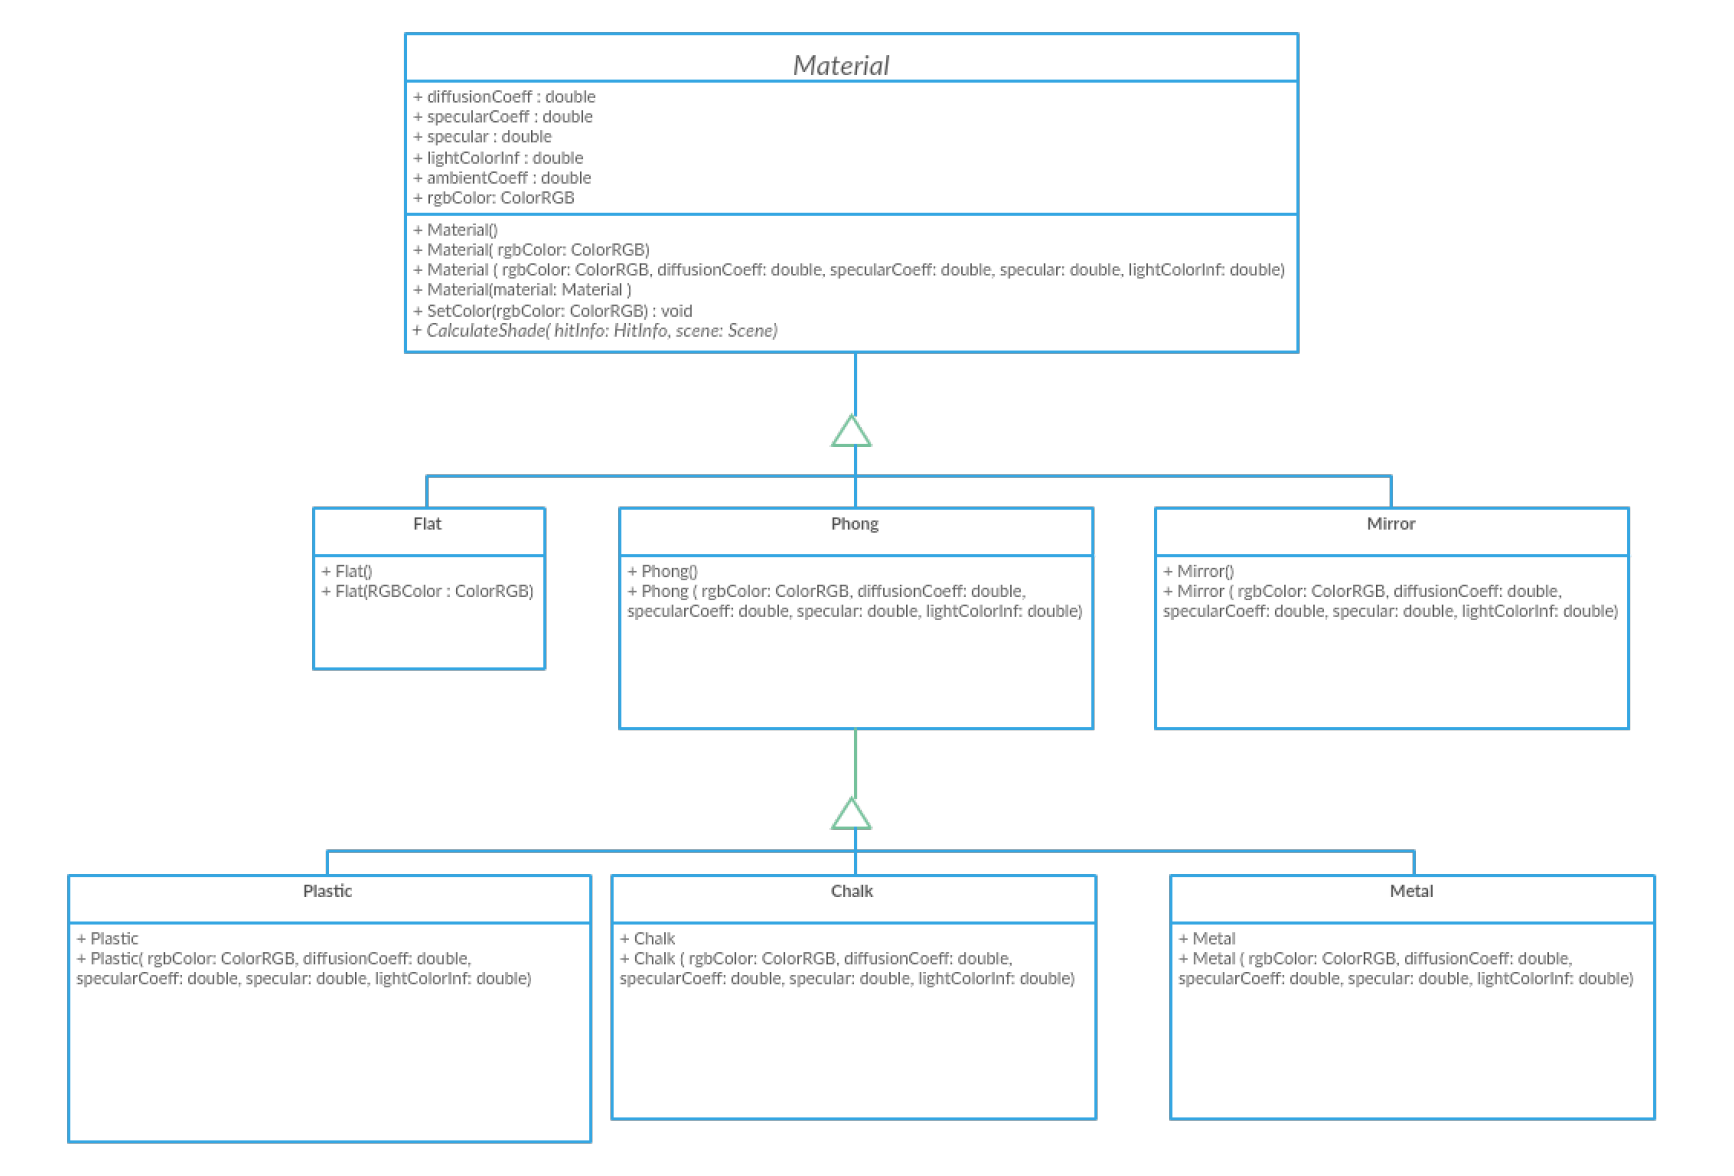
\includegraphics[scale=0.50]{./materials.png}
		\begin{tikzpicture}[scale=0.6, every node/.style={scale=0.7}]
		\umlclass[type=abstract]
		{Material}
		{
			+ diffusionCoeff : double\\
			+ specularCoeff : double\\
			+ specular : double\\
			+ lightColourInf : double\\
			+ ambientCoeff : double\\
			+ rgbColour: ColourRGB
		}
		{
			+ Material() \\
			+ Material( rgbColour: ColourRGB) \\
			+ Material ( rgbColour: ColourRGB, diffusionCoeff: double, \\ \hspace{0.15cm} specularCoeff: double, specular: double, lightColourInf: double)\\
			+ Material(material: Material )\\
			+ SetColour(rgbColour: ColourRGB) : void\\
			+\umlvirt
			{CalculateShade (hitInfo: HitInfo, scene: Scene = null ): HitInfo 
			} 
		} 
		\umlclass[x=0, y=-8.5]{Phong}{}
		{
			+ Phong ()\\
			+ Phong  ( rgbColour: ColourRGB,  \\ \hspace{0.15cm} diffusionCoeff: double, \\ \hspace{0.15cm} specularCoeff: double,  \\ \hspace{0.15cm} specular: double, \\ \hspace{0.15cm} lightColourInf: double)\\
		}
		\umlclass[x=7.2, y=-8.5]{Flat}{}
		{
			+ Flat() \\ 
			+ Flat(RGBColour : ColourRGB)
		} 
		\umlclass[x=-7.2, y=-8.5]{Mirror}{}
		{
			+ Mirror () \\
			+ Mirror ( \\  \hspace{0.15cm} rgbColour: ColourRGB = WHITE,  \\ \hspace{0.15cm} diffusionCoeff: double = 1.0, \\ \hspace{0.15cm} specularCoeff: double = 0.5 ,  \\ \hspace{0.15cm} specular: double = 1.0, \\ \hspace{0.15cm} lightColourInf: double = 0.01)\\
		}
		\umlclass[x=-7, y=-14.5]{Chalk}{}
		{
			+ Mirror () \\
			+ Mirror ( \\  \hspace{0.15cm} rgbColour: ColourRGB,  \\ \hspace{0.15cm} diffusionCoeff: double = 0.4, \\ \hspace{0.15cm} specularCoeff: double = 0.2 ,  \\ \hspace{0.15cm} specular: double = 2.0, \\ \hspace{0.15cm} lightColourInf: double = 0.25)\\
		}
		\umlclass[x=0, y=-14.5]{Plastic}{}
		{
			+ Mirror () \\
			+ Mirror ( \\  \hspace{0.15cm} rgbColour: ColourRGB, \\ \hspace{0.15cm} diffusionCoeff: double = 0.4, \\ \hspace{0.15cm} specularCoeff: double = 0.2 ,  \\ \hspace{0.15cm} specular: double = 20, \\ \hspace{0.15cm} lightColourInf: double = 0.35)\\
		}
		\umlclass[x=7, y=-14.5]{Metal}{}
		{
			+ Mirror () \\
			+ Mirror ( \\  \hspace{0.15cm} rgbColour: ColourRGB, \\ \hspace{0.15cm} diffusionCoeff: double = 0.4 \\ \hspace{0.15cm} specularCoeff: double = 0.2 ,  \\ \hspace{0.15cm} specular: double = 100, \\ \hspace{0.15cm} lightColourInf: double = 0.001)\\
		}
		\umlVHVinherit{Phong}{Material} 
		\umlVHVinherit{Flat}{Material} 
		\umlVHVinherit{Mirror}{Material} 
		\umlVHVinherit{Chalk}{Phong} 
		\umlVHVinherit{Plastic}{Phong} 
		\umlVHVinherit{Metal}{Phong} 
		\end{tikzpicture}
		\caption{Materials Class Diagram}
		\label{fig:matcd}
	\end{figure}
	\subsubsection{Geometry Objects}
	\label{sssec:geo}From the basic idea of ray tracing, we need a method to test whether a ray intersects with the object or not, and since we need our program to be scalable and open for extension, we created an abstract class called geometry object, which will have an attribute called the material; because each object will have a material. In addition to an abstract method called intersect. \newline
	\par In order to add a new geometry object, we need to add a new class, which inherits the GeometryObject abstract class. Then add the attributes needed for the new class, and finally implement the intersect abstract method. The intersect returns an object of type \textbf{HitInfo} which will include the following attributes:
	\begin{itemize}
		\item \textbf{hasHit}: boolean attribute which be \textbf{true} if the ray hits the object, and \textbf{false} if not.
		\item \textbf{hitPoint}: it will be the point of where the ray hit the object. This value will be \textbf{ignored} if \textbf{hasHit} is \textbf{false}.
		\item \textbf{normalAtHit}: it will be the vector which is perpendicular to the hitPoint. This value will be \textbf{ignored}, if \textbf{hasHit} is \textbf{false}.
		\item \textbf{Ray}: it will be the ray which hits the object. This value will be \textbf{ignored}, if \textbf{hasHit} is \textbf{false}.
		\item \textbf{hitObject}: it will be the object which was hit by the ray. This value will be \textbf{ignored}, if \textbf{hasHit} is \textbf{false}.
		\item \textbf{tMin}: it will be smallest value, which is greater than some epsilon value, from many different possible values, that will be produced when a ray hits an object. It will be used to calculate the \textbf{hitPoint}, and it will be \textbf{ignored}, if \textbf{hasHit} is \textbf{false}.
	\end{itemize}
	%I need to add a class diagram for this part
	\par In our program, we have three different objects as illustrated in \textbf{Figure \ref{fig:geo}}. Each of these objects has its own attributes, in addition to one of the supported materials, which were listed in \textbf{Section \ref{sssec:mat}}.
	\begin{figure}[ht!]
		\centering
		%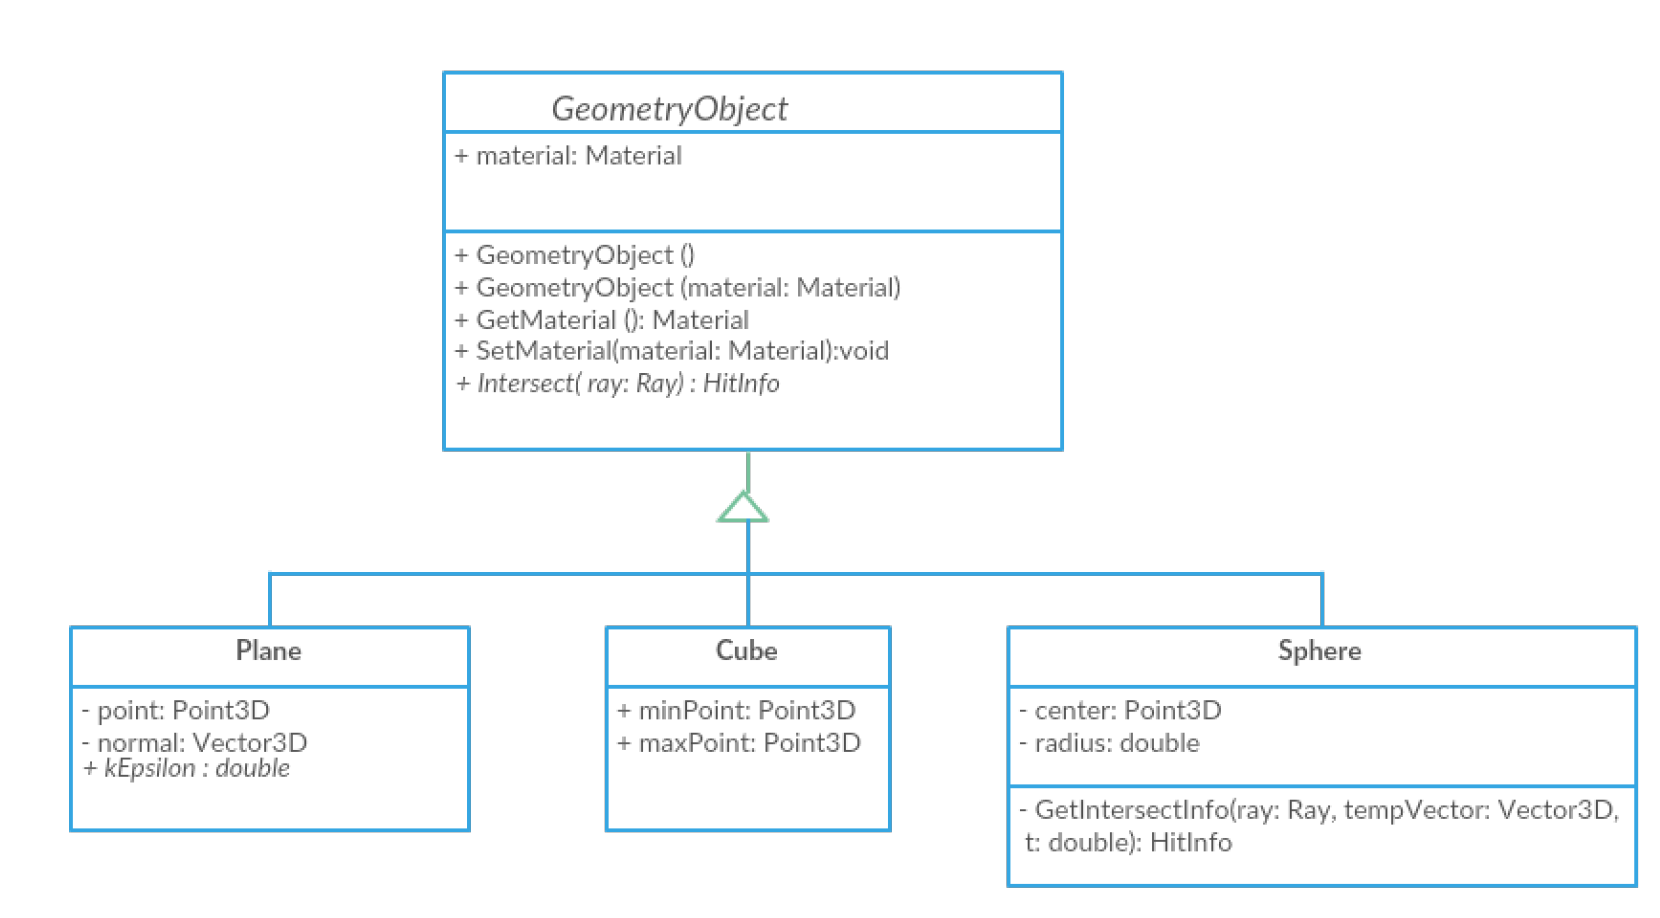
\includegraphics[scale=0.50]{./objects.png}
		\begin{tikzpicture} [scale=0.75, every node/.style={scale=0.75}]
		\umlclass[type=abstract]
		{GeometryObject}
		{+ material : Material}
		{
			+ GeometryObject () \\ 
			+ GeometryObject (material: Material) \\ 
			+ GetMaterial (): Material \\ 
			+ SetMaterial (material: Material): void \\ 
			+ \umlvirt{Intersect (ray: Ray): HitInfo } 
		} 
		\umlclass[x=0, y=-5]{Sphere}
		{ - center: Point3D \\ - radius: double} 
		{
			- GetIntersectInfo(ray: Ray, \\ tempVector: Vector3D, t: double): HitInfo 
		}
		\umlclass[x=6, y=-5]{Cube}{+ minPoint: Point3D \\ + maxPoint: Point3D}{} 
		\umlclass[x=-6, y=-5]{Plane}{
			- point: Point3D \\ 
			- normal: Vector3D \\ 
			+ \textit{kEpsilon : double} 
		}{} 
		\umlVHVinherit{Sphere}{GeometryObject} 
		\umlVHVinherit{Cube}{GeometryObject} 
		\umlVHVinherit{Plane}{GeometryObject} 
		\end{tikzpicture}
		\caption{Geometry Objects Class Diagram}
		\label{fig:geo}
	\end{figure}
	\subsubsection{Lights}
	\label{sssec:light}Each light will have a colour, intensity and a position. There might be different types of lights, and that's why we created a class called \textbf{Light}, and it is not an abstract class; since we want to create instances of it. Therefore, we defined it is method to be virtual, and so they can be overridden if we need to change their default implementation. The methods in this class are:
	\begin{itemize}
		\item \textbf{GetDistance}: this method will calculate the distance between some point, and the position of the light.         \item \textbf{GetDirection}: this method will calculate the direction of the light with respect to some given point.
		\item \textbf{GetColour}: this method will calculate the final colour after considering the light effects, such as the colour and intensity.
	\end{itemize}
	\subsubsection{Tracer}
	The tracer class will be responsible for tracing an input ray with all objects in the scene. Then, if the ray hits one of the objects, it will recursively call the method for some predefined depth value. Then, it will use the hitInfo in order to call the \textbf{CalculateShade} method, which was previously discussed in the materials section, and the \textbf{TraceShadeRay} method, which will calculate the effects of lights on the object.\newline
	\par Finally, the result will be the multiplication of the values returned by the previous two methods in case the ray hits one of the objects, otherwise, it will be the colour of the scene's background.
	\subsubsection{Camera}
	\label{sssec:cam} Another important element of ray tracing is the camera, which represents the way of looking to the objects in the scene. There are many different types of cameras that can be used such as perspective and orthographic cameras. In our implementation, we decided to make our application as simple as possible for end-users and as a result, we chose to only implement the perspective camera. This choice means that the user can set the camera to be a certain distance from the scene, thus giving them the ability to zoom in and out unlike with the orthographic camera where there is no distance from the scene.
	
	In order to keep our program open for any future extension, we created an abstract class called camera, which contains:
	\begin{itemize}
		\item \textbf{Attributes}:
		\begin{itemize} 
			\item \textbf{Position}: which is a 3D point represents the position of the camera in the scene.
			\item \textbf{lookAt}: which is a 3D vector represents the direction of how to look at the scene.
		\end{itemize}
		\item \textbf{Methods and Operations}: These methods will be implemented differently based on the type of the camera
		\begin{itemize} 
			\item \textbf{Render()}: this method will be doing the ray tracing algorithm, by going through all pixels in the window frame and get the colour of that pixel.
			\item \textbf{FindRayDirection(Point2D point)} : this method will calculate the ray direction from a given point in the window frame with respect to the camera's values.
		\end{itemize}
	\end{itemize}
	\par In the perspective camera's implementation, the \textbf{Render} loops through all pixels in the image plane,  and then calculate the point, which will be used as an input to \textbf{FindRayDirection} method, and then call the \textbf{TraceRay}, which was discussed before in the previous section. 
	\subsubsection{Sampling}
	To make the resulting colour smoother, we used one of the sampling techniques called the regular sampling technique. In our application, we used the \textbf{Regular Sampling Technique}. The main idea is to do the tracing on the same square of the image plane, but at different sampling values, and calculate the colour at different points inside that square for \textbf{N \footnote{The number of samples}} times.\newline
	\par Finally, we sum up these values together and divide the result by \textbf{N} which will be the final colour of that square. By applying this technique, the final colour will be smoother than not utilising any sampling technique at all.
	\subsubsection{Scene}
	The scene will be the container of all the previously mentioned classes. Each scene will have a list of geometry objects, list of lights, camera, background colour, sampler, file name which will be the final name of the output file.\newline
	\par The scene will also have many different methods:
	\begin{itemize}
		\item \textbf{GetHitInfo}: This method will find if the ray hits any of the objects in the scene, and will return the hitInfo of the nearest object which was hit by the ray, in addition to other values of hitInfo, which were discussed before in \textbf{Section \ref{sssec:geo}}.
		\item \textbf{Render}: it will call the render method of the camera's object. More details about this method can be found in \textbf{Section \ref{sssec:cam}}.
		\item \textbf{DisplayPixel}: it will take the x and y indices of a point, with the calculated colour as inputs, and then assign that colour to the appropriate index in the final picture pixels result.
		\item \textbf{FinalPicture}: this method will just print the colours in the final pixels array, which are filled by the \textbf{DisplayPixel}, that is called by the \textbf{Render} method, into an image of jpg type, with the filename received from the front end.
	\end{itemize}
	\subsection{Controllers}
	In our project, we have one controller called \textbf{RenderController}, that will act as a POST API. It will receive a JSON from the front end side, the responsibility of that controller is to parse the received JSON, in a way that can be understood by the back end's implementation. That's why we are having JSON folder in our project.\newline
	\par The parsing process is done by a method called \textbf{ProcessJSON} in \textbf{JSONObject} class. We need this class as an interpreter between the front and back ends; since the way the front end deals with the environment and object values is not the same as the back end. Therefore, for simplicity and to avoid doing a lot of processing calculations and computations on the client side, it is done on the back end side.\newline
	\par After parsing the JSON to the appropriate format, we can create the scene object by then calling the \textbf{Render} method. This method requires time to render the whole scene.The bigger the scene and the number of objects and lights, the more time it takes for the scene to render. After that \textbf{FinalPicture} method is called, to finally return the image to the front end as JPG file.
	\subsection{Testing}\label{sec:backend-tests}
	In the back end, we made a decision to write unit tests to cover the main and critical functionality of our system. We used the \textbf{NUnit} package in order to write our tests. In this section, we will discuss the importance of unit testing, and the details of implementing it.\newline
	\par In our tests, we tested whether each operation returned the expected result. It was crucial to test many different operations in our program, such as the addition, subtraction, scaling, dot and cross products in addition to other operations for the elements model. Also, the main operations in lights, sampling, tracing, materials, and the intersect methods in all geometry objects are in the same level of importance to be tested.\newline
	\par In fact, it is good to mention that not all the tests are straightforward; since some methods are calling other methods. Therefore, we wrote \textbf{SceneTest} class, where this class overrides some of the methods to return custom values based on the scenario we are testing. Also, we made use of the mock objects, where we can control what a method should return based on some input without executing the actual implementation of it. Examples of this can be seen in Scene testing.
	\section{Front End}
	One of the main objectives of the project was to create a product that is easy and intuitive to use. In order to enable users to define the various elements they wish to have rendered on the scene, a simple web interface was developed. The interface allows users to enter the different values for the scene elements such as objects with different materials, positions, sizes and colours. Furthermore, the interface allows the user to define the specifications of the scene, even allowing them to add multiple lights at different positions with different colours and intensities.\newline 
	\par The web interface has two main modes. One mode shows a 2D representation of the scene and is comprised of two views; a top down and a side view. The 2D view is useful because it allows the user to accurately position the objects in the scene with easy since the camera is always static and only from two different perspectives. The shortcoming of the 2D view is that even though it gives the user the ability to position elements exactly as they want, the user has to continuously imagine and think about how their scene will actually look in the end. Furthermore, the different lighting and camera positions that the user has configured are not rendered in the 2D views. The 3D view, on the other hand, does allow the user to rotate around the scene and see how objects are positioned in every dimension at once whilst also showing a rough approximation of what the ray traced scene is going to look like. 
	\subsection{Set up}
	In order to make sure we followed good engineering practices and allowed our code to be easily extendable, we implemented the entire client in ES6 styled JavaScript. ES6 is quickly becoming an industry standard with the rise of \textit{NodeJS} and \textit{TypeScript} and thanks to its modularity, forces us into a neat pattern around which we can structure our codebase. What is more, because ES6 JavaScript can be run both locally and in the browser, we were able to implement extensive testing using the \textit{Mocha.js} testing framework and incorporate granular unit tests into our continuous integration pipeline - we expand on our front end testing process in section \ref{sec:frontend-tests}.\newline
	\par Though adoption is ever growing, ES6 JavaScript is not supported by a number of current browsers and therefore we chose to transpile and bundle our code using \textit{Browserify} into browser runnable JavaScript. To avoid us having to continuously re-package the bundled code manually we utilised a hot module replacement tool called \textit{Watchify}. \textit{Watchify} monitored each of our included dependencies and whenever changes were saved to a file, the bundle would immediately be rebuilt, ready for us to see our code in action. The combination of an ES6 codebase, hot module replacement, bundling and good unit test coverage made developing the project a frictionless affair.
	
	\subsection{SVG} \label{sec:svg}
	
	The first couple iterations of the project from the client side focused on creating a simple user interface that allows the user to input the most basic objects and parameters for the scene. By taking this approach we'd guarantee to be delivering a functional product from early in the project lifecycle. As we began development, it was immediately obvious that we had to decide on standards that can be used to represent the scene and the objects being rendered in a concise yet expressive way. During our first meeting we created and documented a  \href{https://github.com/davidbenicek/raytracer/wiki/Initial-JSON-payload-design}{\underline{\textit{JSON structure}}} that would be used to hold the render request and sent from the front end to the back end.\newline
	
	\par The very first task was to implement the kind of prototype you see in Figure \ref{fig:firstIt}. By starting with just a simple form page we enabled ourselves to verify some of the assumptions we made about the JSON structure and the kind of controls we were planning on presenting to the user. While parts of the form were going to change in subsequent iterations, we established a way to harvest the values from any form by developing a generic function that takes a class name and strips out the values from child inputs of the target class and saves them in a JSON. This piece of code is instrumental to how the front end client works and was used throughout development, including in the final solution - see \href{https://github.com/davidbenicek/raytracer/blob/e85055df16c4534989220de84ce67656a276bf33/src/RayTracer/Public/js/form.js#L30}{\underline{\textit{form.js}}} for the code.\newline 
	
	In one of the early iterations, we also implemented the \textit{sendToApi.js} file which is responsible for the communication with the back end. The file has evolved over time as the interface between the two parts of the system changed, however, it's main role has remained the same. The main objective of the functions within the sendToApi module is to sanitise the output of the front end, send a POST request with the resulting JSON that represents the user's input to the back end and receive and save the ray traced image. 
	
	\par Once we had a simple interface that allowed us to send the simplest configuration possible (simple scene and one object) to be the back end, it was time to make the product more user-friendly. The first step was to create two 2D views (top down and side view) to allow the user to get an idea of what the scene they were rendering would look like in terms of colour and position. There was some debate about how to implement the 2D views, including the usage of some third party libraries but we opted to use a completely custom solution using SVG since it would give us the freedom of defining its exact behaviour and appearance. During this iteration the second pivotal set of functions was implemented - the JSON to SVGs converting function that can be found in \href{https://github.com/davidbenicek/raytracer/blob/e85055df16c4534989220de84ce67656a276bf33/src/RayTracer/Public/js/render.js#L43}{\underline{\textit{render.js}}}. The aim of these functions is to take each of the object expressed in the JSON and create equivalent SVG objects and place them into the SVG canvas. The main focus while writing these functions was extensibility and therefore if you examine the code you'll see that all that is needed to implement an extra shape is to define a getSVGFor\textit{object} function that would then be called based on the execution of the switch statement inside convertToSvg. Even though we did not manage to implement other objects apart from a cube and sphere, this could be easily achieved in the future. \newline
	
	
	\par One of the best features the front end has is the support for dragging and dropping elements. This feature enables users to interact with the product in a familiar way and enables them to add multiple objects to the scene without having to key in the values for their positions into a long and hard to understand form. The drag and drop functionality was also implemented from scratch to allow us to customise the behaviour and fine tune it to our expectations. The code was loosely inspired by the work of Collingridge \cite{collingridge_draggable_2011}, however, our solution is more complex and refined than his. The implementation of the feature was difficult because it involved dragging an object from one SVG (the itinerary on top in Figure \ref{fig:drag_drop}) into the main canvas below it, which is itself a different SVG. \newline
	
	\begin{figure}[ht!]
		\centering
		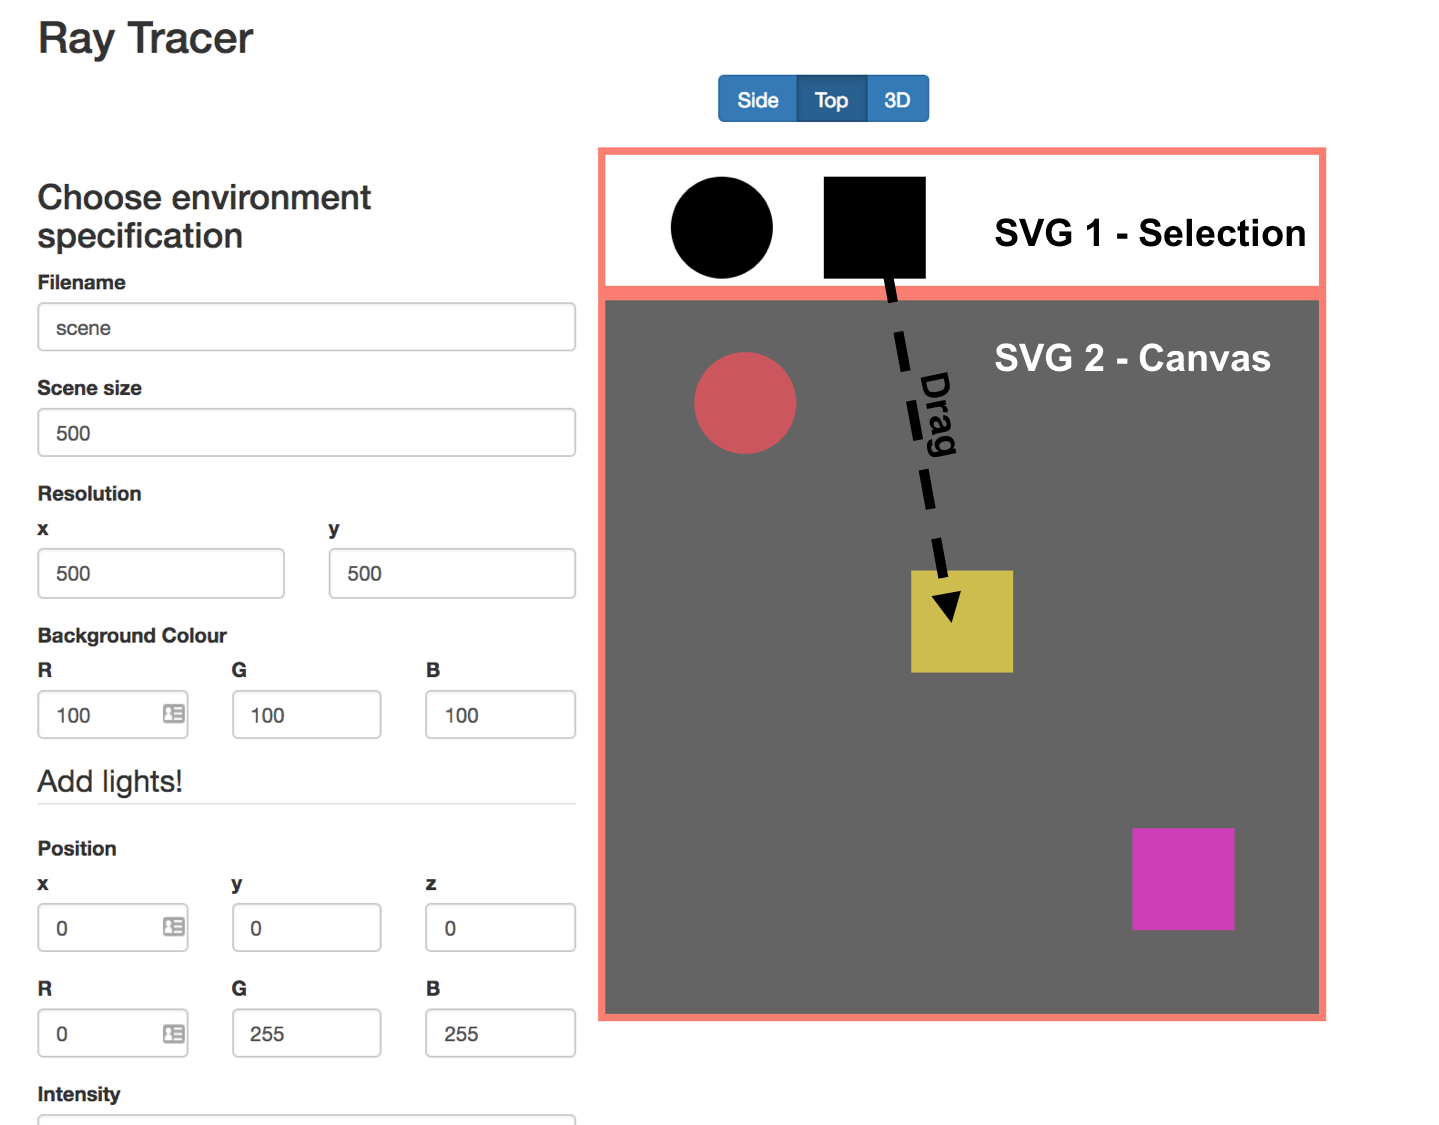
\includegraphics[scale=0.30]{drag.png}
		\caption{Screenshot to illustrate the drag and drop functionality}
		\label{fig:drag_drop}
	\end{figure}
	
	
	\par The final piece to the puzzle was creating a feature that allows the user to modify individual objects once they are on the scene. We decided to implement a tooltip that appears when an element is double-clicked as seen below in Figure \ref{fig:tooltip}. The solution for the tooltip is again completely custom made and works similarly to the initial version of the form, except that its values are always populated depending on which object is clicked and during the harvesting of the values we save them such that they override the correct object details rather than limiting the JSON to being only one object.
	
	\begin{figure}[ht!]
		\centering
		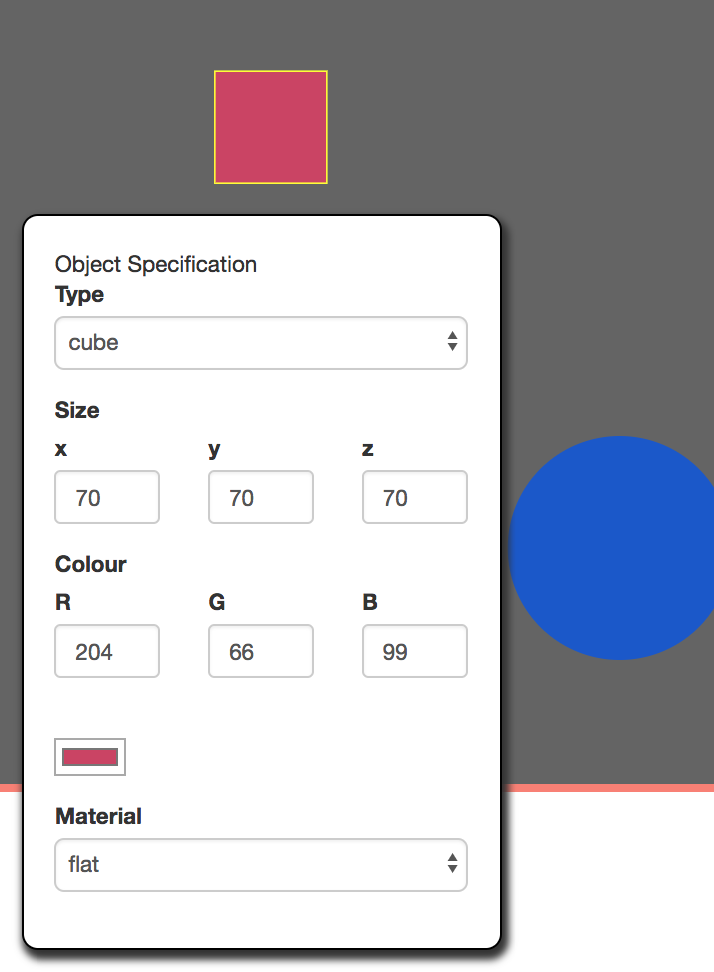
\includegraphics[scale=0.30]{tooltip.png}
		\caption{Screenshot of tooltip}
		\label{fig:tooltip}
	\end{figure}
	
	\subsection{3D}
	The 3D is used to give the user an approximation of the image that will be produced by the back end. The 3D view was developed using a JavaScript library called Three(three.js)\cite{three.js_three.js_2018}. Three is a combination of SVG and WebGL with a simpler way to create objects and all the other necessities such as clicking and labelling. This API is well known as diverse companies\cite{three.js_three.js_2018} such as Toyota, Porsche or even Google \cite{google_rubiks_2014} use it.\newline
	
	\par Three is quite similar to our back end as the majority of the functions that the back end provides can be simulated in Three. Functions like adding different materials; adding lights with different intensities and colours; and obviously having a 3D aspect. The difference is, this library allows the user to rotate the scene which can then help them decide how they want the ray tracing image to look like. For example, one user might like an angle better than the other or another user will like the camera position to be higher or lower than the normal view. This gives the user more freedom as opposed to having those two parameters set as default in the background or just having a 2D view which would not be an actual representation.\newline 
	
	\par Rendering the 3D scene was quite straightforward, this was due to the fact that every time an element was added to the scene, it was saved to a JSON. The JavaScript file implementing the three read the JSON and added objects and lights according to the users' input. It also changed the values of the scene and lights if the user wanted to change them while they were viewing the 3D scene. This was done using JQuery which allowed a "refresh" of the scene without loading the page again and inputting all the elements from scratch. Reading the JSON and adding the elements to the scene was simple as well because the Three library had all of these elements predefined already. Therefore, all we had to do was create functions that would add the certain element to the scene by just getting the values from the JSON. There are 2 different functions in the file. One is to add the lights to the scene and the other is to add the shape to the scene which would then call another function depending on the users choice of shape. Having the file read the JSON made applying this library to our front end simple and also it reassured us that the JSON was coded in the right format as this same JSON was then sent to the back end to render the same exact scene.
	
	\subsection{Testing} \label{sec:frontend-tests}
	\par One of the strengths of ES6 Javascript is that it enables developers to code in a very modular way. The general approach we took was to have different features separated over individual files with one exported module per file. Thanks to this structure, testing was quite easy. We have multiple tests files, each importing the module it is testing. A decision was made to leave out front end dependant code from the test coverage because this would involve either simulating a DOM or at least simulating our interactions with the DOM both of which have quite a high up front cost in terms of set up time. Due to the relative simplicity of the code and the brevity of the project, this upfront investment of time and effort would likely not yield much interest in the short time the project is run for. \newline
	\par The testing was carried out using a testing framework called \textit{Chai.js}, which works on a basis of assertions that can either pass or fail. Periodically, we would use a tool called \textit{Istanbul} to run a coverage report to get an idea of how much of our code base is being visited during the tests. The test coverage differed on a file by file basis, mostly determined by how much background logic and how much DOM interaction happened within the code of a given file. Some files, such as render.js, have 100\% statement coverage because they are completely independent of the DOM and contain important logic that determines how different objects are rendered as SVG elements. Other files, such as render-3d.js, that are heavily dependant both on DOM interactions and external libraries have far lower test coverage.\newline
	
	\chapter{Team work}\label{chapter:teamwork}
	%In this section: Describe how you worked together, including the tools and processes you used to facilitate group work.
	\section{Process} \label{sec:process}
	
	We decided early on to establish weekly meetings to reinforce communication and collaboration within the group. The structure of the meetings changed as time went on and as we learnt more about optimising our meeting efficiency. We initially started by adopting the "walk the board" method where we would run through the issues in the current sprint and talk about the status of each issue \cite{schlabach_agile_2009}. This is generally a useful technique, however, it led us into a pattern of only mentioning work done on the specific issues and not always mentioning any extra work done which created a knowledge gap in the team. After the initial presentation, we decided to abandon the walk the board approach and instead adopted a format whereby each member of the group would explain what they had achieved over the past week and the others would provide feedback. Often the summary would relate directly to the individual issues just as before but sometimes we would exchange extra information which previously went unheard. After each member took their turn updating the team we would discuss and decide what needed to be accomplished by the next week. Each weekly meeting produced weekly targets to streamline progress on the project, these targets would often be converted into Github issues which is discussed below. These meetings also gave us the opportunity to assist each other on areas where we might be having difficulty and very often the group would continue to work together after the meetings in the same vein as pair programming. Working and coding together as a group helped us become more productive and had the added benefit of allowing us to bond.\newline
	\par Outside of our physical meetings we took advantage of messaging services like Whatsapp and Facebook Messenger to stay in touch and Gruveo for online meetings (more on this below).\newline
	
	\par Working in Agile was extremely beneficial to the team as we had frequent release cycles (iterations) and therefore also weekly feedback on our work. This effectively allowed for quality assurance testing to be done on each cycle, so defects were found early on as opposed to being discovered at the end of the project. The flexibility of Agile allowed us to update requirements and shift priorities at the beginning of each cycle, guiding the team in their work for the next iteration. Thanks to Agile's focus on\textit{working deliverables} (as opposed to \textit{perfect deliverables}) we were able to fulfil the basic requirements of the project faster, giving us more time to concentrate on additional features.\newline
	
	\par There are also downsides to using Agile in that the method splits the work into individual components that needed to be later combined together unlike a progressive system with a clear start and finish. This had the side effect of creating addition responsibilities for the transitions between the individual models so that they could be edited together into a cohesive system.
	
	
	
	\section{Communication}
	Communication is one of the most important factors when it comes to working in a software engineering team. For our project, we decided to utilise a number of different structured and unstructured communication channels. There exists a large array of great project management and issue tracking tools such as JIRA, Trac or Trello, however, we decided that given the brevity of our project and the relative low number of backlog items (especially at the start), that it would be best to keep our ticket system as close to the codebase as possible. As a result of this, we decided to make use of the inbuilt GitHub issue tracking system. This system does not provide the same calibre of project management tools as some of the aforementioned products, however, it does enough for our purposes. We decided to use the GitHub milestone system as a way of scheduling issues for our sprints and implemented a branch naming convention such that we would refer to the issues we are addressing in the name of the branch - \{issue number\}/\{name of branch\}. This simple mechanism has worked tremendously; because it ensures that on one hand all branches are addressing exactly one task or feature and on the other hand, that all tasks and features have been recorded in an issue. \newline
	\par Another way we structured our communication was by the use of pull requests whenever pushing code to master. By raising a pull request and having another team member review it, we not only improved our code quality but also spread knowledge of the code base and cross-pollinated ideas for features and more efficient solutions. Standout examples of a pull request flow can be seen \href{https://github.com/davidbenicek/raytracer/pull/36}{\underline{\textit{here (pull request \#36)}}} and \href{https://github.com/davidbenicek/raytracer/pull/66}{\underline{\textit{here (pull request \#66)}}}\newline
	
	\par Not all communication can be done over issue summaries and pull requests and therefore we scheduled weekly meetings to go over what has been achieved, what needs to be discussed and what is the plan for the following sprint. One could say that we condensed our daily scrum meeting, sprint planning, backlog refinement and sprint review all into one weekly meeting. This is not the textbook way of running an Agile project but given that we are not working on the project full time and that these meetings were kept as brief as possible, it still aligns to the core principles of Agile. During the meetings, we would discuss the general trajectory of the project and what we want to accomplish in the next seven days, before breaking off into our sub-teams and deciding on the exact issues we needed to create for the week ahead. Towards the end of the project, workload increased, therefore it was important to have two meetings per week to make sure everyone was on track and knew what they were doing. This way of running a project has both advantages and disadvantages, which is covered in section \ref{sec:process}. We mostly met in person but on occasion, when we needed to, we used video conferencing tools such as Appear.In and Gruveo to connect with each other when team members were unavailable to meet during the week.\newline
	
	
	During the course of the sprints, our communication did not fade. We built on some ideas from Extreme Programming and met frequently in our work units to engage in pair programming while working on issues during the sprint. To facilitate the smooth operation of the team we used the lowest friction medium of communication for all of us which was a WhatsApp group where we have discussed everything from meeting times, the status of different issues or even specific lines of code in a pull request. 
	
	\section{Tools} \label{sec:tools}
	Various tools were used by us, in order to build our final product. These tools will be discussed in this section in further details.
	\subsection{Software Development Tools}
	\subsubsection{Visual Studio}
	IDE from Microsoft that our back end team used in the development of the main ray tracing components, supporting our coding in C\#. It was key in helping us implement and maintain the MVC model. Visual Studio offers many helpful features, including a code editor supporting IntelliSense \footnote{The code completion component}, as well as code refactoring and an integrated debugger.
	\subsubsection{Visual Studio Code}
	The source code editor that the front end team mainly used, offers a plethora of beneficial features as it includes support for debugging, embedded Git control, syntax highlighting, intelligent code completion, snippets, and code refactoring. 
	\subsection{Project Management Tools}
	Management is a very important key for a project to succeed, and since we all believe in that, we used different tools to manage and organise our work. 
	\subsubsection{Git}
	Git was used as our version control software. This helped us manage our source code, keep track of files and store a complete history of our code base. It also helped us create tickets to improve goal setting as explained above. The project was versioned controlled using GitHub.
	\subsubsection{Travis CI}
	It is a continuous integration service that we used to build and test the code whenever it was pushed up to GitHub. 
	\subsubsubsection{Mocha}
	Mocha is a JavaScript testing framework that we used for further testing of our code (mainly on the front end). It features browser support, asynchronous testing, test coverage reports and allows developers to use an assertion library to test their co. \cite{dzone_mocha_2018}
	\subsection{Communication Tools}
	
	The main tools we used to stay in touch outside of our physical meetings was \textbf{Whatsapp} and to a lesser extent \textbf{Facebook Messenger}. We set up a group with everyone in it on Whatsapp and relied on both Facebook and Whatsapp for direct messaging. These messaging services allowed us to query each other anytime we had a question about the project or when we needed information from one of our team members. This ease of contact helped decrease the amount time that we spent stuck on problems as we could quickly rely on each other should any problem arise. The WhatsApp group also made group announcements easier ensuring everyone was up to date on the project progress and direction.\newline
	\par\textbf{Gruveo} enabled us to have online video conferences for those instances when we weren't available to meet in person (e.g. when a group member was abroad). It doesn't require any sign up so the team leader just had to send a link in the group and everyone was able to join the call with ease.
	
	\chapter{Evaluation}
	\section{Our work}
	Throughout the life cycle of the project we encountered both a number of challenges that throttled our progress and discovered things that were easier than initially expected. Considering the mandatory requirements that were set out at the onset of the project, all of them have been accomplished. Furthermore, we managed to complete most of our optional requirements except for allowing the users to input extra objects like polygons since we choose to implement a plane object instead. We made sure to structure the code base such that it was easily extensible and therefore, if it wasn't for the project deadline serving as a time constraint, it would be trivial to implement more custom objects since we would be able to simply extend and inherit a lot of the functionality that we have already implemented. \newline
	
	\par As described in Chapter \ref{chapter:teamwork}, the team was divided into two. This was largely a success as each team member decided whether they wanted to work on either the front end or the back end depending on their own skills, desires or work experience. This was crucial as everyone chose the area they were more comfortable working with which allowed fewer issues to arise in the future. Each sub-team also had at least one member who had work experience in the particular field. David had experience in front end development, whereas Othman had experience working with back end systems. This was important as both of them were able to lead their sub-team and any problems would be solved efficiently. It also gave the rest of the team members a look into the future as both of their experience helped the team visualise and learn how different code practices and tools such as testing suites or linting software are used in the workplace. Despite some of these tools having steep learning curves it was a worthwhile investment of our time because in the long run, they allowed us to work more efficiently and to better software engineering standards as described in section \ref{sec:tools}. Another aspect that went well is being able to always have meetings. There were times that some group members had to travel but meetings were never cancelled. We always worked a way around it, either by scheduling the meeting to another day or by having the meeting through video calls instead of face to face. We also decided to have two meetings per week as the workload increased at the end and more reviewing, team work was required by one another. If tasked to complete the project again, it would be interesting to see what effect, if any, there would be on the functioning of the team if we had rotated individuals between the sub-teams. Such an experiment may lead to more cross-pollination of ideas and could serve the team well if carried out well. \newline 
	
	
	\par Focusing on the mandatory requirements first seemed logical as they were the functionality required for the software to work. Once those were accomplished, the optional requirements would be prioritised. This process went well as we did manage to finish the mandatory requirements. Most of the mandatory tasks were divided into the sub-teams which lead to both individual work and working in pairs. Critical tasks such as SVG implementation on the front end or creating different shapes in the back end, was either developed through pair programming or each team member had a small task to do in them, for example, one team member would create a cube and the other a sphere. This helped us participate in every aspect of the project and improved our skills such as teamworking and communication. This also led to coding problems being solved quickly as two minds are quicker and more knowledgeable than one. On the other hand, small tasks that were also important such as fixing a bug or creating forms were done individually as not much time was needed for them.  \newline
	
	\par Communication within a team can often be a challenging and frustrating task, especially at early stages of team formation. As described by Tuckman, groups usually go through a number of stages namely forming, storming and norming before finally reaching a stage where the team can operate efficiently and effectively \cite{tuckman_development_1965} and this could not be more true for our team. At the beginning of the project, all of us started with an optimistic mindset and were eager to begin. We made an effort at the beginning to plan and coordinate our future actions by creating prototypes (\ref{sec:prototypes}), establishing interfaces(\ref{sec:svg}) and eliciting requirements (\ref{chapter:requirements}) however this proved to not be enough. As weeks passed and we dove deeper into the project, we encountered problems and questions that we had not previously answered as a team. This uncertainty and lack of forward planning led to individuals making well intentioned decisions (often the correct ones) but not doing a good enough job at communicating these slight course adjustments back to the rest of the team. The result was unsurprising. At the time of the initial presentation, we arrived as two systems - a front end and a back end, that had deviated from one another, not in major ways but in slight details that made the two systems incompatible. The issues faced were indeed trivial (Amercian versus British spelling conventions, differentiating default values of variables etc.) however, they were indicative of a larger issue in team communication.\newline
	
	\par As we scrambled to integrate the two systems, just days and hours before the presentation, it was clear that this was not the correct way forward. Fortunately, there was ample time to improve our communication as a team. Immediately after the presentation, we came up with a number of actions and policies that would keep us on track and enforce a healthy level of communication and integration policing. The steps, outlined in our \href{https://github.com/davidbenicek/raytracer/wiki/5th-Meeting-(14th-Feb-2018)}{\underline{\textit{meeting minutes}}}, included restructuring the code base to better fit with our architecture, setting up a continuous integration system and changing the structure of our team meetings to be more action-oriented rather than issue focused as described in Section \ref{sec:process}. Changing the way we worked halfway through the project was not a comfortable task and definitely made us go through a storming period within the team, however, the processes yielded great results and taught us valuable lessons not only for this project but also for our future endeavours. In the future, we could consider adopting weekly or bi-weekly retrospectives which would allow the team to self-critique its process from within and perhaps uncover dysfunctional parts of our process quicker. \newline
	
	\par Teams are frequently faced with difficult dilemmas about their processes that boil down to whether it is worth investing time and effort in the short term in order to harvest the benefits further down the development cycle. For long-lasting teams. it is generally a good idea to invest in establishing things such as testing suites or rigorous coding standard because in the long term they are likely to benefit from these early investments. When it comes to short-term projects, especially at university, this can be a tricky decision to make. Under invest in your development practices and you get caught up in spaghetti code, over commit and you end up with a great, clean code base but no end product. In our team, we decided that it was important for us to have the main program logic and interfaces covered by unit and integration tests respectively. The different parts of the system that were covered, as well as the rationale for these decisions,  can be found in sections \ref{sec:backend-tests} and \ref{sec:frontend-tests}. Our approach served us well, especially in the back end because we had a defined process thanks to taking guidance from the book \cite{suffern_ray_2007} and therefore we simply kept building atop individual functions. In the front end, however, as we iterated and implemented varying functionalities we could have done with better test coverage. At the start we made a decision not to test functions that involved interacting directly with the DOM as this seemed too extensive, especially given the brevity of the project, however later on our code started to rely more and more on front end interactions and therefore this is something we should have considered more closely. \newline
	
	\par If given a chance to start again, it would be beneficial for us to implement some sort of front end testing or at least mocking/stubbing tests to simulate DOM interactions. Using libraries such as Selenium we could have simulated user interactions in the browser and ran these as part of our CI pipeline rather than having to rely on manual testing as we did. On one or two occasions we accepted breaking changes coming into master because weren't able to cover all scenarios of UI interactions during manual inspections and having automated browser tests would have prevented this. Another option to test our front end dependant code would have been to mock the interactions of our code with the DOM by using a library such as Sinon to stub the functions that interact with the rendered elements and make them return different results, which would simulate user interactions without having to launch the code in a browser. In an ideal scenario and in a longer-term project, we would implement both of these techniques and run them as often as possible to ensure we are not introducing any breaking changes during development. By having unit tests, integration tests and browser tests, we would be adhering to the notion of the test pyramid \cite{vocke_practical_2018}, having a couple large, slow test that examine the system on an end to end basis and plenty of fast, granular unit tests that test the code in isolation, hopefully guaranteeing a healthy code base.\newline
	
	\par At the start of each sprint, we would hold a sprint planning session during which each team member would commit to complete a number of tasks before the next meeting. Seeing as everyone was working on the project only part-time, there was a high probability that external issues such as deadlines for other courses or holidays may impact individuals ability to complete the work on time and impact the schedule of the project. We aimed to plan our work with this in mind and often had to re-assign issues to other members when individuals struggled to finish their tasks. Generally, this mechanism worked as members owned up to their decreased throughput in one sprint and worked harder to improve their track record in the following weeks. Knowing that scheduling can be difficult, we went as far as setting an internal deadline for the main parts of the code to be done by the 28th of February in order to have plenty of time to write the final report due at the end of March. As is frequently the case with software engineering, "the first 90 percent of the code accounts for the first 90 percent of the development time. The remaining 10 percent of the code accounts for the other 90 percent of the development time" \cite{bentley_programmimg_1985} and we ended up having to push back the deadline by a week in order to complete all the requirements with some small and final bug fixing continuing throughout March. The decision to set an internal deadline far ahead of the official deadline was perhaps one of the best choices we made as a team; because it decreased pressure at the end of the project and allowed us to exert a constant amount of effort over time rather than having to rely on a spike in effort at the end.\newline
	
	\section{Future Work}
	
	\par Projects, especially in the computer industry can be never-ending. One can argue that a ray tracer falls into this category, as there are always new features that can be implemented to make the ray tracer better, faster and more complete. One of the many features could be to add different shapes. There are numerous shapes that we have not touched upon and adding a greater number of shapes can make this ray tracer unique. However, this is challenging as these shapes need to be showcased in both 2D and 3D in the front end, and then again in 3D in the back end. The reason why this is challenging is that a lot of the shapes are not similar to one another, therefore each aspect of the shapes would have to be created from scratch, which is both difficult and time consuming. Additionally, another future feature could be allowing the user the freedom to create their own shape by letting them sketch it out, for example, consider drawing a shape in 2D in Microsoft Paint and then allowing the back end to form a 3D version of it. A new feature of our product could be a new technology that replaces our 3D library. This feature could give a more accurate representation of the back end without sending the values. This is not possible with the current technologies available to us. An ideal feature would be having a library that allows the exact same ray tracer that we are using in the back end to be shown in the web page. This feature would make it completely accurate and would satisfy the customers.There are also improvements that could be made in the front end.\newline
	
	\par There is always a trade-off between a simple and clean user interface and over-complication. However, there are certainly ways in which we could improve. Small adjustments such as including a colour picker next to all colour selection input rather than just the objects ones or making some input boxes into sliders could already significantly improve both the aesthetic of the interface and its ease of use. Other future improvements could also include making the user interface more friendly towards disabled users by making sure we specify correct alt text for screen readers, using high contrast colours for the colour blind and enabling the entire page to be operated using just keyboard operations for users with low dexterity. \newline
	
	\par The product we made is customizable, while that makes the product more user-friendly and it gives the user the freedom to have the scene in any way they want, it also has its limitations. The main limitation we have is that most of the values that the user inputs will not produce a scene with all of the objects being perfectly visible in the scene. This is an issue as the user will have to do trial and error until they get the perfect value. This can be solved by allowing the user to input the type of scene they want and the back end being able to calculate the correct camera position, camera angle or even the scene size. The perfect values would then be sent to the user and they would then be able to use those values without spending too much time on it. \newline
	
	\par  Overall, the project has been a great learning experience for each of us as individuals and we have managed to accomplish a significant amount while successfully achieving the main aim of the project. The experience learnt in this project will help us do better in the future projects, especially in those projects that require working in a team.
	
	%In this section: Critically evaluate your project: what worked well, and what didn’t? how did you do relative to your plan? what changes were the result of improved thinking and what changes were forced upon you? how did your team work together? etc. Note that you need to show that you understand the weaknesses in your work as well as its strengths. You may wish to identify relevant future work that could be done on your project.
	
	\section{Peer Assessment}
	\begin{table}[ht!]
		\begin{center}
			\caption{Peer Assessment}
			\resizebox{\textwidth}{!}{%
				\begin{tabular}{|l|l|l|l|l|l|l|}
					\hline
					\textbf{Member}         & Othman Alkhamra & David Benicek & Hitesh Mankani Vinod & Timothy Obimma & Aadam Bari & Nagarjuna Vaddiraju \\ \hline
					\textbf{Student Number} & 1756850         & 1739256       & 1425704             & 1755013        & 1770922    & 1783087             \\ \hline
					\textbf{Marks}          & 22.37           & 22.37         & 17.08               & 17.08          & 13.4       & 7.7                 \\ \hline
				\end{tabular}%
			}
		\end{center}
	\end{table}
	\clearpage
	\bibliographystyle{plainurl}
	\bibliography{references}
\end{document}